% Options for packages loaded elsewhere
\PassOptionsToPackage{unicode}{hyperref}
\PassOptionsToPackage{hyphens}{url}
\PassOptionsToPackage{dvipsnames,svgnames,x11names}{xcolor}
%
\documentclass[
  letterpaper,
  DIV=11,
  numbers=noendperiod]{scrartcl}

\usepackage{amsmath,amssymb}
\usepackage{iftex}
\ifPDFTeX
  \usepackage[T1]{fontenc}
  \usepackage[utf8]{inputenc}
  \usepackage{textcomp} % provide euro and other symbols
\else % if luatex or xetex
  \usepackage{unicode-math}
  \defaultfontfeatures{Scale=MatchLowercase}
  \defaultfontfeatures[\rmfamily]{Ligatures=TeX,Scale=1}
\fi
\usepackage{lmodern}
\ifPDFTeX\else  
    % xetex/luatex font selection
\fi
% Use upquote if available, for straight quotes in verbatim environments
\IfFileExists{upquote.sty}{\usepackage{upquote}}{}
\IfFileExists{microtype.sty}{% use microtype if available
  \usepackage[]{microtype}
  \UseMicrotypeSet[protrusion]{basicmath} % disable protrusion for tt fonts
}{}
\makeatletter
\@ifundefined{KOMAClassName}{% if non-KOMA class
  \IfFileExists{parskip.sty}{%
    \usepackage{parskip}
  }{% else
    \setlength{\parindent}{0pt}
    \setlength{\parskip}{6pt plus 2pt minus 1pt}}
}{% if KOMA class
  \KOMAoptions{parskip=half}}
\makeatother
\usepackage{xcolor}
\setlength{\emergencystretch}{3em} % prevent overfull lines
\setcounter{secnumdepth}{-\maxdimen} % remove section numbering
% Make \paragraph and \subparagraph free-standing
\ifx\paragraph\undefined\else
  \let\oldparagraph\paragraph
  \renewcommand{\paragraph}[1]{\oldparagraph{#1}\mbox{}}
\fi
\ifx\subparagraph\undefined\else
  \let\oldsubparagraph\subparagraph
  \renewcommand{\subparagraph}[1]{\oldsubparagraph{#1}\mbox{}}
\fi

\usepackage{color}
\usepackage{fancyvrb}
\newcommand{\VerbBar}{|}
\newcommand{\VERB}{\Verb[commandchars=\\\{\}]}
\DefineVerbatimEnvironment{Highlighting}{Verbatim}{commandchars=\\\{\}}
% Add ',fontsize=\small' for more characters per line
\usepackage{framed}
\definecolor{shadecolor}{RGB}{241,243,245}
\newenvironment{Shaded}{\begin{snugshade}}{\end{snugshade}}
\newcommand{\AlertTok}[1]{\textcolor[rgb]{0.68,0.00,0.00}{#1}}
\newcommand{\AnnotationTok}[1]{\textcolor[rgb]{0.37,0.37,0.37}{#1}}
\newcommand{\AttributeTok}[1]{\textcolor[rgb]{0.40,0.45,0.13}{#1}}
\newcommand{\BaseNTok}[1]{\textcolor[rgb]{0.68,0.00,0.00}{#1}}
\newcommand{\BuiltInTok}[1]{\textcolor[rgb]{0.00,0.23,0.31}{#1}}
\newcommand{\CharTok}[1]{\textcolor[rgb]{0.13,0.47,0.30}{#1}}
\newcommand{\CommentTok}[1]{\textcolor[rgb]{0.37,0.37,0.37}{#1}}
\newcommand{\CommentVarTok}[1]{\textcolor[rgb]{0.37,0.37,0.37}{\textit{#1}}}
\newcommand{\ConstantTok}[1]{\textcolor[rgb]{0.56,0.35,0.01}{#1}}
\newcommand{\ControlFlowTok}[1]{\textcolor[rgb]{0.00,0.23,0.31}{#1}}
\newcommand{\DataTypeTok}[1]{\textcolor[rgb]{0.68,0.00,0.00}{#1}}
\newcommand{\DecValTok}[1]{\textcolor[rgb]{0.68,0.00,0.00}{#1}}
\newcommand{\DocumentationTok}[1]{\textcolor[rgb]{0.37,0.37,0.37}{\textit{#1}}}
\newcommand{\ErrorTok}[1]{\textcolor[rgb]{0.68,0.00,0.00}{#1}}
\newcommand{\ExtensionTok}[1]{\textcolor[rgb]{0.00,0.23,0.31}{#1}}
\newcommand{\FloatTok}[1]{\textcolor[rgb]{0.68,0.00,0.00}{#1}}
\newcommand{\FunctionTok}[1]{\textcolor[rgb]{0.28,0.35,0.67}{#1}}
\newcommand{\ImportTok}[1]{\textcolor[rgb]{0.00,0.46,0.62}{#1}}
\newcommand{\InformationTok}[1]{\textcolor[rgb]{0.37,0.37,0.37}{#1}}
\newcommand{\KeywordTok}[1]{\textcolor[rgb]{0.00,0.23,0.31}{#1}}
\newcommand{\NormalTok}[1]{\textcolor[rgb]{0.00,0.23,0.31}{#1}}
\newcommand{\OperatorTok}[1]{\textcolor[rgb]{0.37,0.37,0.37}{#1}}
\newcommand{\OtherTok}[1]{\textcolor[rgb]{0.00,0.23,0.31}{#1}}
\newcommand{\PreprocessorTok}[1]{\textcolor[rgb]{0.68,0.00,0.00}{#1}}
\newcommand{\RegionMarkerTok}[1]{\textcolor[rgb]{0.00,0.23,0.31}{#1}}
\newcommand{\SpecialCharTok}[1]{\textcolor[rgb]{0.37,0.37,0.37}{#1}}
\newcommand{\SpecialStringTok}[1]{\textcolor[rgb]{0.13,0.47,0.30}{#1}}
\newcommand{\StringTok}[1]{\textcolor[rgb]{0.13,0.47,0.30}{#1}}
\newcommand{\VariableTok}[1]{\textcolor[rgb]{0.07,0.07,0.07}{#1}}
\newcommand{\VerbatimStringTok}[1]{\textcolor[rgb]{0.13,0.47,0.30}{#1}}
\newcommand{\WarningTok}[1]{\textcolor[rgb]{0.37,0.37,0.37}{\textit{#1}}}

\providecommand{\tightlist}{%
  \setlength{\itemsep}{0pt}\setlength{\parskip}{0pt}}\usepackage{longtable,booktabs,array}
\usepackage{calc} % for calculating minipage widths
% Correct order of tables after \paragraph or \subparagraph
\usepackage{etoolbox}
\makeatletter
\patchcmd\longtable{\par}{\if@noskipsec\mbox{}\fi\par}{}{}
\makeatother
% Allow footnotes in longtable head/foot
\IfFileExists{footnotehyper.sty}{\usepackage{footnotehyper}}{\usepackage{footnote}}
\makesavenoteenv{longtable}
\usepackage{graphicx}
\makeatletter
\def\maxwidth{\ifdim\Gin@nat@width>\linewidth\linewidth\else\Gin@nat@width\fi}
\def\maxheight{\ifdim\Gin@nat@height>\textheight\textheight\else\Gin@nat@height\fi}
\makeatother
% Scale images if necessary, so that they will not overflow the page
% margins by default, and it is still possible to overwrite the defaults
% using explicit options in \includegraphics[width, height, ...]{}
\setkeys{Gin}{width=\maxwidth,height=\maxheight,keepaspectratio}
% Set default figure placement to htbp
\makeatletter
\def\fps@figure{htbp}
\makeatother

\usepackage{array}
\usepackage{caption}
\usepackage{graphicx}
\usepackage{siunitx}
\usepackage[normalem]{ulem}
\usepackage{colortbl}
\usepackage{multirow}
\usepackage{hhline}
\usepackage{calc}
\usepackage{tabularx}
\usepackage{threeparttable}
\usepackage{wrapfig}
\usepackage{adjustbox}
\usepackage{hyperref}
\KOMAoption{captions}{tableheading}
\makeatletter
\makeatother
\makeatletter
\makeatother
\makeatletter
\@ifpackageloaded{caption}{}{\usepackage{caption}}
\AtBeginDocument{%
\ifdefined\contentsname
  \renewcommand*\contentsname{Table of contents}
\else
  \newcommand\contentsname{Table of contents}
\fi
\ifdefined\listfigurename
  \renewcommand*\listfigurename{List of Figures}
\else
  \newcommand\listfigurename{List of Figures}
\fi
\ifdefined\listtablename
  \renewcommand*\listtablename{List of Tables}
\else
  \newcommand\listtablename{List of Tables}
\fi
\ifdefined\figurename
  \renewcommand*\figurename{Figure}
\else
  \newcommand\figurename{Figure}
\fi
\ifdefined\tablename
  \renewcommand*\tablename{Table}
\else
  \newcommand\tablename{Table}
\fi
}
\@ifpackageloaded{float}{}{\usepackage{float}}
\floatstyle{ruled}
\@ifundefined{c@chapter}{\newfloat{codelisting}{h}{lop}}{\newfloat{codelisting}{h}{lop}[chapter]}
\floatname{codelisting}{Listing}
\newcommand*\listoflistings{\listof{codelisting}{List of Listings}}
\makeatother
\makeatletter
\@ifpackageloaded{caption}{}{\usepackage{caption}}
\@ifpackageloaded{subcaption}{}{\usepackage{subcaption}}
\makeatother
\makeatletter
\@ifpackageloaded{tcolorbox}{}{\usepackage[skins,breakable]{tcolorbox}}
\makeatother
\makeatletter
\@ifundefined{shadecolor}{\definecolor{shadecolor}{rgb}{.97, .97, .97}}
\makeatother
\makeatletter
\makeatother
\makeatletter
\makeatother
\ifLuaTeX
  \usepackage{selnolig}  % disable illegal ligatures
\fi
\IfFileExists{bookmark.sty}{\usepackage{bookmark}}{\usepackage{hyperref}}
\IfFileExists{xurl.sty}{\usepackage{xurl}}{} % add URL line breaks if available
\urlstyle{same} % disable monospaced font for URLs
\hypersetup{
  pdftitle={In-field assays},
  colorlinks=true,
  linkcolor={blue},
  filecolor={Maroon},
  citecolor={Blue},
  urlcolor={Blue},
  pdfcreator={LaTeX via pandoc}}

\title{In-field assays}
\author{}
\date{2023-04-14}

\begin{document}
\maketitle
\ifdefined\Shaded\renewenvironment{Shaded}{\begin{tcolorbox}[boxrule=0pt, interior hidden, borderline west={3pt}{0pt}{shadecolor}, frame hidden, sharp corners, breakable, enhanced]}{\end{tcolorbox}}\fi

\begin{Shaded}
\begin{Highlighting}[]
\FunctionTok{source}\NormalTok{(here}\SpecialCharTok{::}\FunctionTok{here}\NormalTok{(}\StringTok{"setup.R"}\NormalTok{))}
\end{Highlighting}
\end{Shaded}

\begin{verbatim}
Skipping install of 'drcData' from a github remote, the SHA1 (09f9da30) has not changed since last install.
  Use `force = TRUE` to force installation
\end{verbatim}

\begin{verbatim}
Skipping install of 'drc' from a github remote, the SHA1 (8719d43a) has not changed since last install.
  Use `force = TRUE` to force installation
\end{verbatim}

\begin{verbatim}
Skipping install of 'medrc' from a github remote, the SHA1 (bc36df51) has not changed since last install.
  Use `force = TRUE` to force installation
\end{verbatim}

\begin{verbatim}
[conflicted] Will prefer dplyr::filter over any other package.
[conflicted] Will prefer dplyr::select over any other package.
\end{verbatim}

\begin{Shaded}
\begin{Highlighting}[]
\FunctionTok{library}\NormalTok{(lme4)}
\FunctionTok{theme\_set}\NormalTok{(}\FunctionTok{theme\_bw}\NormalTok{(}\AttributeTok{base\_size=}\DecValTok{12}\NormalTok{))}
\end{Highlighting}
\end{Shaded}

\begin{Shaded}
\begin{Highlighting}[]
\NormalTok{dat }\OtherTok{\textless{}{-}}\NormalTok{ rio}\SpecialCharTok{::}\FunctionTok{import}\NormalTok{(}\StringTok{"data/field.csv"}\NormalTok{) }\SpecialCharTok{\%\textgreater{}\%} 
  \FunctionTok{mutate\_at}\NormalTok{(}\FunctionTok{vars}\NormalTok{(fungicide, season, tree), as.factor) }\SpecialCharTok{\%\textgreater{}\%} 
  \FunctionTok{mutate}\NormalTok{(}\AttributeTok{fungicide=}\FunctionTok{fct\_relevel}\NormalTok{(fungicide, }\StringTok{"Control"}\NormalTok{))}
\FunctionTok{str}\NormalTok{(dat)}
\end{Highlighting}
\end{Shaded}

\begin{verbatim}
'data.frame':   60 obs. of  5 variables:
 $ fungicide: Factor w/ 3 levels "Control","Bellis",..: 1 1 1 1 1 1 1 1 1 1 ...
 $ season   : Factor w/ 2 levels "1","2": 2 2 2 2 2 2 2 2 2 2 ...
 $ tree     : Factor w/ 10 levels "1","2","3","4",..: 1 2 3 4 5 6 7 8 9 10 ...
 $ leaves   : int  250 250 250 250 250 250 250 250 250 250 ...
 $ diseased : int  27 19 26 30 16 40 27 22 19 8 ...
\end{verbatim}

Data scheme

\begin{Shaded}
\begin{Highlighting}[]
\FunctionTok{ftable}\NormalTok{(}\FunctionTok{xtabs}\NormalTok{(}\SpecialCharTok{\textasciitilde{}}\NormalTok{ fungicide }\SpecialCharTok{+}\NormalTok{ tree }\SpecialCharTok{+}\NormalTok{ season, dat))}
\end{Highlighting}
\end{Shaded}

\begin{verbatim}
               season 1 2
fungicide tree           
Control   1           1 1
          2           1 1
          3           1 1
          4           1 1
          5           1 1
          6           1 1
          7           1 1
          8           1 1
          9           1 1
          10          1 1
Bellis    1           1 1
          2           1 1
          3           1 1
          4           1 1
          5           1 1
          6           1 1
          7           1 1
          8           1 1
          9           1 1
          10          1 1
Ziram     1           1 1
          2           1 1
          3           1 1
          4           1 1
          5           1 1
          6           1 1
          7           1 1
          8           1 1
          9           1 1
          10          1 1
\end{verbatim}

Model

\begin{Shaded}
\begin{Highlighting}[]
\NormalTok{dat }\SpecialCharTok{\%\textgreater{}\%} 
  \FunctionTok{ggplot}\NormalTok{() }\SpecialCharTok{+} 
  \FunctionTok{aes}\NormalTok{(}\AttributeTok{x=}\NormalTok{fungicide, }\AttributeTok{y=}\NormalTok{diseased}\SpecialCharTok{/}\NormalTok{leaves) }\SpecialCharTok{+} 
  \CommentTok{\# geom\_boxplot(width=.5) + }
  \FunctionTok{geom\_text}\NormalTok{(}\FunctionTok{aes}\NormalTok{(}\AttributeTok{label=}\NormalTok{tree))}\SpecialCharTok{+}
  \FunctionTok{geom\_jitter}\NormalTok{(}\AttributeTok{width=}\NormalTok{.}\DecValTok{2}\NormalTok{, }\AttributeTok{col=}\DecValTok{2}\NormalTok{, }\AttributeTok{alpha=}\NormalTok{.}\DecValTok{5}\NormalTok{) }\SpecialCharTok{+} 
  \FunctionTok{labs}\NormalTok{(}\AttributeTok{x=}\StringTok{"Treatment"}\NormalTok{, }\AttributeTok{y=}\StringTok{"Disease incidence"}\NormalTok{) }\SpecialCharTok{+} 
  \FunctionTok{facet\_wrap}\NormalTok{(}\StringTok{"season"}\NormalTok{)}
\end{Highlighting}
\end{Shaded}

\begin{figure}[H]

{\centering 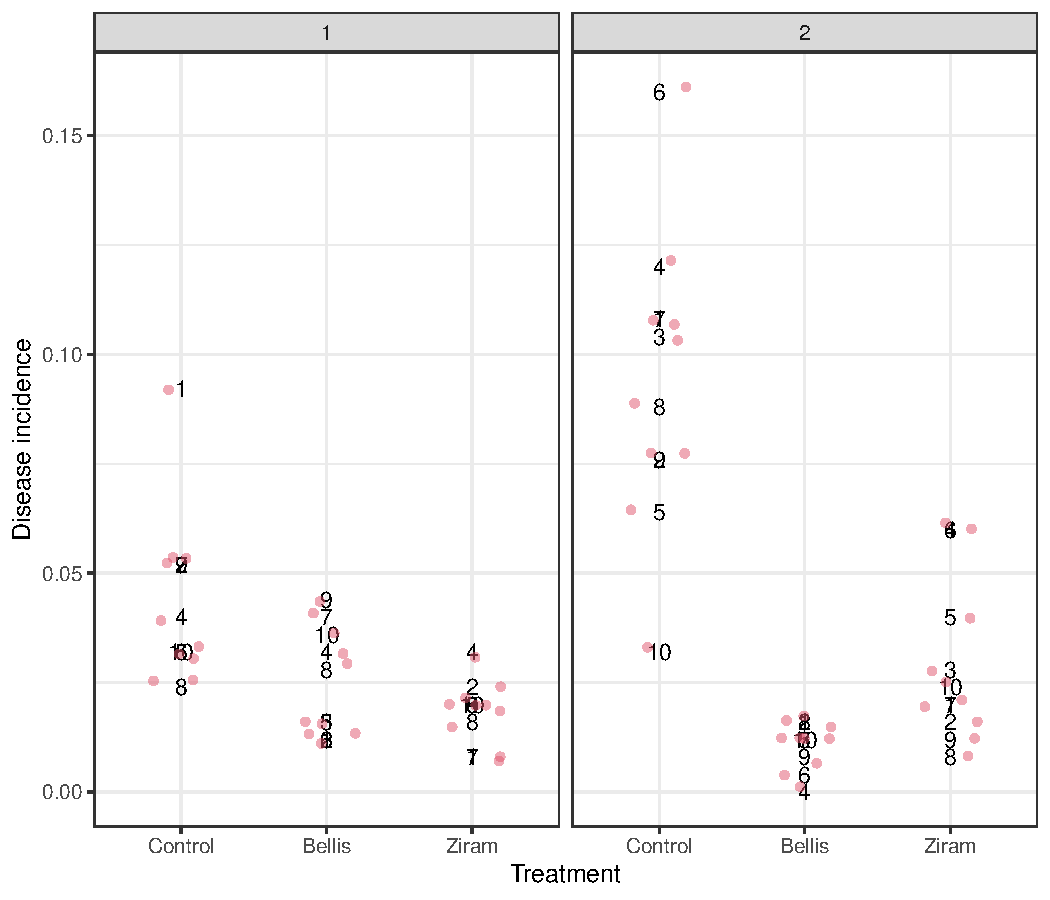
\includegraphics{in_field_files/figure-pdf/unnamed-chunk-4-1.pdf}

}

\end{figure}

\begin{Shaded}
\begin{Highlighting}[]
\NormalTok{mod }\OtherTok{\textless{}{-}} \FunctionTok{glmer}\NormalTok{(diseased}\SpecialCharTok{/}\NormalTok{leaves }\SpecialCharTok{\textasciitilde{}}\NormalTok{ fungicide }\SpecialCharTok{*}\NormalTok{ season }\SpecialCharTok{+}\NormalTok{ (}\DecValTok{1}\SpecialCharTok{|}\NormalTok{tree),}
             \AttributeTok{weights=}\NormalTok{leaves, }\AttributeTok{family=}\NormalTok{binomial, dat)}
\end{Highlighting}
\end{Shaded}

Goodness of fit

\begin{Shaded}
\begin{Highlighting}[]
\FunctionTok{simulateResiduals}\NormalTok{(mod) }\SpecialCharTok{\%\textgreater{}\%} \FunctionTok{testResiduals}\NormalTok{()}
\end{Highlighting}
\end{Shaded}

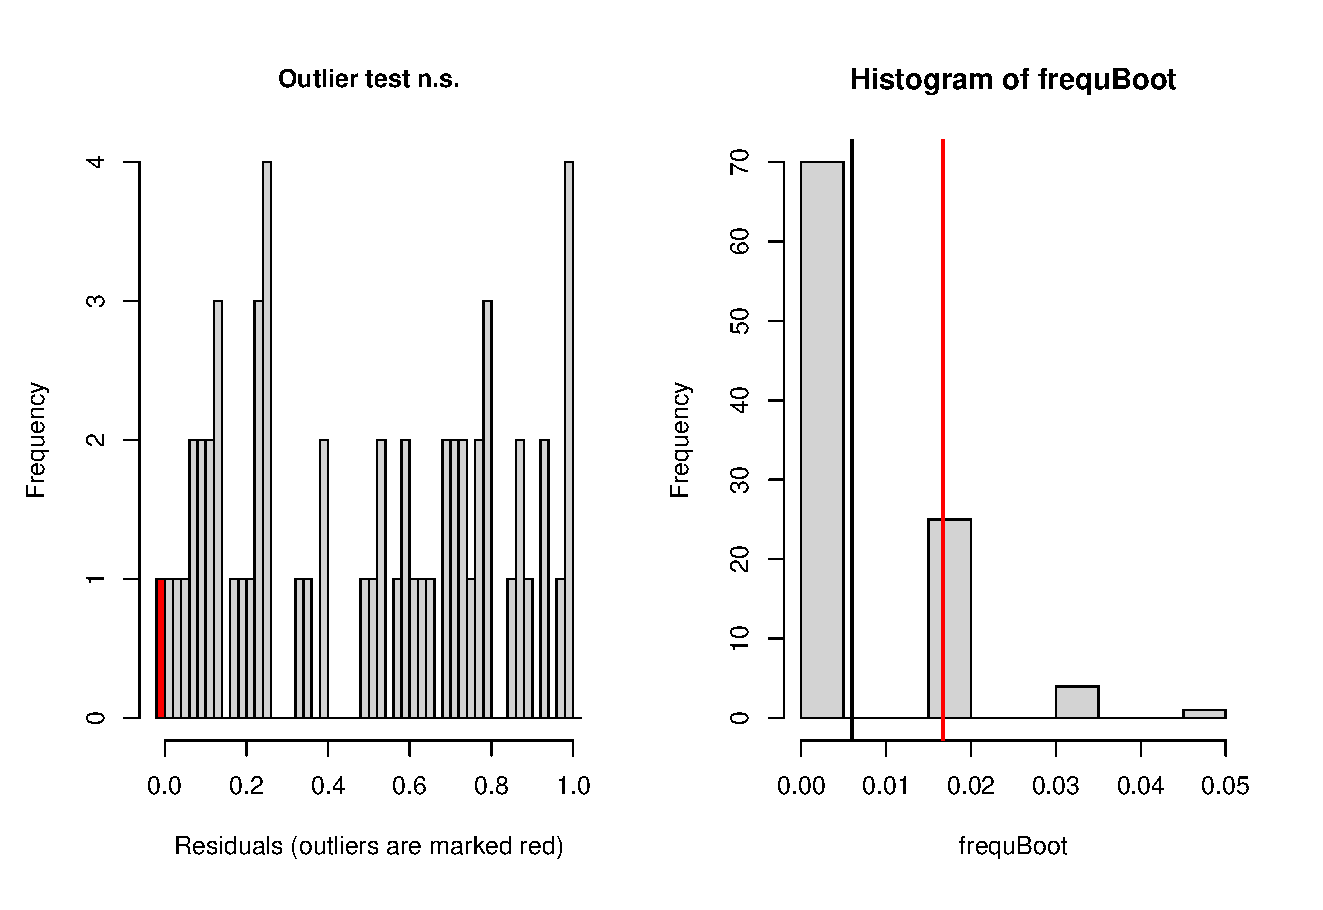
\includegraphics{IN FIELD.eps}

\begin{Shaded}
\begin{Highlighting}[]
\NormalTok{car}\SpecialCharTok{::}\FunctionTok{Anova}\NormalTok{(mod)}
\end{Highlighting}
\end{Shaded}

 
  \providecommand{\huxb}[2]{\arrayrulecolor[RGB]{#1}\global\arrayrulewidth=#2pt}
  \providecommand{\huxvb}[2]{\color[RGB]{#1}\vrule width #2pt}
  \providecommand{\huxtpad}[1]{\rule{0pt}{#1}}
  \providecommand{\huxbpad}[1]{\rule[-#1]{0pt}{#1}}

\begin{table}[ht]
\begin{centerbox}
\begin{threeparttable}
 
\setlength{\tabcolsep}{0pt}
\begin{tabular}{l l l}


\hhline{>{\huxb{0, 0, 0}{0.4}}->{\huxb{0, 0, 0}{0.4}}->{\huxb{0, 0, 0}{0.4}}-}
\arrayrulecolor{black}

\multicolumn{1}{!{\huxvb{0, 0, 0}{0.4}}r!{\huxvb{0, 0, 0}{0}}}{\huxtpad{6pt + 1em}\raggedleft \hspace{6pt} \textbf{Chisq} \hspace{6pt}\huxbpad{6pt}} &
\multicolumn{1}{r!{\huxvb{0, 0, 0}{0}}}{\huxtpad{6pt + 1em}\raggedleft \hspace{6pt} \textbf{Df} \hspace{6pt}\huxbpad{6pt}} &
\multicolumn{1}{r!{\huxvb{0, 0, 0}{0.4}}}{\huxtpad{6pt + 1em}\raggedleft \hspace{6pt} \textbf{Pr($>$Chisq)} \hspace{6pt}\huxbpad{6pt}} \tabularnewline[-0.5pt]


\hhline{>{\huxb{0, 0, 0}{0.4}}->{\huxb{0, 0, 0}{0.4}}->{\huxb{0, 0, 0}{0.4}}-}
\arrayrulecolor{black}

\multicolumn{1}{!{\huxvb{0, 0, 0}{0.4}}r!{\huxvb{0, 0, 0}{0}}}{\cellcolor[RGB]{242, 242, 242}\huxtpad{6pt + 1em}\raggedleft \hspace{6pt} 161\hphantom{0}\hphantom{0} \hspace{6pt}\huxbpad{6pt}} &
\multicolumn{1}{r!{\huxvb{0, 0, 0}{0}}}{\cellcolor[RGB]{242, 242, 242}\huxtpad{6pt + 1em}\raggedleft \hspace{6pt} 2 \hspace{6pt}\huxbpad{6pt}} &
\multicolumn{1}{r!{\huxvb{0, 0, 0}{0.4}}}{\cellcolor[RGB]{242, 242, 242}\huxtpad{6pt + 1em}\raggedleft \hspace{6pt} 1.35e-35 \hspace{6pt}\huxbpad{6pt}} \tabularnewline[-0.5pt]


\hhline{>{\huxb{0, 0, 0}{0.4}}|>{\huxb{0, 0, 0}{0.4}}|}
\arrayrulecolor{black}

\multicolumn{1}{!{\huxvb{0, 0, 0}{0.4}}r!{\huxvb{0, 0, 0}{0}}}{\huxtpad{6pt + 1em}\raggedleft \hspace{6pt} 25.2 \hspace{6pt}\huxbpad{6pt}} &
\multicolumn{1}{r!{\huxvb{0, 0, 0}{0}}}{\huxtpad{6pt + 1em}\raggedleft \hspace{6pt} 1 \hspace{6pt}\huxbpad{6pt}} &
\multicolumn{1}{r!{\huxvb{0, 0, 0}{0.4}}}{\huxtpad{6pt + 1em}\raggedleft \hspace{6pt} 5.11e-07 \hspace{6pt}\huxbpad{6pt}} \tabularnewline[-0.5pt]


\hhline{>{\huxb{0, 0, 0}{0.4}}|>{\huxb{0, 0, 0}{0.4}}|}
\arrayrulecolor{black}

\multicolumn{1}{!{\huxvb{0, 0, 0}{0.4}}r!{\huxvb{0, 0, 0}{0}}}{\cellcolor[RGB]{242, 242, 242}\huxtpad{6pt + 1em}\raggedleft \hspace{6pt} 41.1 \hspace{6pt}\huxbpad{6pt}} &
\multicolumn{1}{r!{\huxvb{0, 0, 0}{0}}}{\cellcolor[RGB]{242, 242, 242}\huxtpad{6pt + 1em}\raggedleft \hspace{6pt} 2 \hspace{6pt}\huxbpad{6pt}} &
\multicolumn{1}{r!{\huxvb{0, 0, 0}{0.4}}}{\cellcolor[RGB]{242, 242, 242}\huxtpad{6pt + 1em}\raggedleft \hspace{6pt} 1.18e-09 \hspace{6pt}\huxbpad{6pt}} \tabularnewline[-0.5pt]


\hhline{>{\huxb{0, 0, 0}{0.4}}->{\huxb{0, 0, 0}{0.4}}->{\huxb{0, 0, 0}{0.4}}-}
\arrayrulecolor{black}
\end{tabular}
\end{threeparttable}\par\end{centerbox}

\end{table}
 

Means comparison test

\begin{Shaded}
\begin{Highlighting}[]
\NormalTok{emm }\OtherTok{\textless{}{-}} \FunctionTok{emmeans}\NormalTok{(mod, }\SpecialCharTok{\textasciitilde{}}\NormalTok{ fungicide}\SpecialCharTok{|}\NormalTok{season, }\AttributeTok{type=}\StringTok{"response"}\NormalTok{) }
\NormalTok{res }\OtherTok{\textless{}{-}} \FunctionTok{cld}\NormalTok{(emm, }\AttributeTok{alpha=}\FloatTok{0.05}\NormalTok{, }\AttributeTok{Letters=}\NormalTok{letters,  }\AttributeTok{type=}\StringTok{"response"}\NormalTok{) }\SpecialCharTok{\%\textgreater{}\%} 
   \FunctionTok{mutate}\NormalTok{(}\StringTok{\textasciigrave{}}\AttributeTok{\%Control}\StringTok{\textasciigrave{}}\OtherTok{=}\FunctionTok{abs}\NormalTok{((prob}\SpecialCharTok{/}\NormalTok{dplyr}\SpecialCharTok{::}\FunctionTok{filter}\NormalTok{(.,fungicide}\SpecialCharTok{==}\StringTok{"Control"}\NormalTok{)}\SpecialCharTok{\%\textgreater{}\%} \FunctionTok{pull}\NormalTok{(prob)}\SpecialCharTok{{-}}\DecValTok{1}\NormalTok{)}\SpecialCharTok{*}\DecValTok{100}\NormalTok{)) }\SpecialCharTok{\%\textgreater{}\%} 
\NormalTok{  tibble}

\NormalTok{res }\SpecialCharTok{\%\textgreater{}\%} 
  \FunctionTok{rename}\NormalTok{(}\AttributeTok{Season=}\StringTok{"season"}\NormalTok{) }\SpecialCharTok{\%\textgreater{}\%} 
  \FunctionTok{ggplot}\NormalTok{()}\SpecialCharTok{+}
  \FunctionTok{aes}\NormalTok{(}\AttributeTok{x=}\NormalTok{fungicide, }\AttributeTok{y =}\NormalTok{prob)}\SpecialCharTok{+}
  \FunctionTok{geom\_pointrange}\NormalTok{(}\FunctionTok{aes}\NormalTok{(}\AttributeTok{ymin=}\NormalTok{asymp.LCL , }\AttributeTok{ymax=}\NormalTok{asymp.UCL))}\SpecialCharTok{+}
  \FunctionTok{facet\_wrap}\NormalTok{(}\StringTok{"Season"}\NormalTok{, }\AttributeTok{labeller =}\NormalTok{ label\_both) }\SpecialCharTok{+} \FunctionTok{geom\_text}\NormalTok{(}\FunctionTok{aes}\NormalTok{(}\AttributeTok{label=}\FunctionTok{str\_squish}\NormalTok{(.group)), }\AttributeTok{angle=}\DecValTok{90}\NormalTok{, }\AttributeTok{vjust=}\SpecialCharTok{{-}}\DecValTok{1}\NormalTok{, }\AttributeTok{hjust=}\NormalTok{.}\DecValTok{5}\NormalTok{, ) }\SpecialCharTok{+} 
  \FunctionTok{geom\_jitter}\NormalTok{(}\AttributeTok{data=}\NormalTok{dat}\SpecialCharTok{\%\textgreater{}\%}\FunctionTok{rename}\NormalTok{(}\AttributeTok{Season=}\StringTok{"season"}\NormalTok{) , }\FunctionTok{aes}\NormalTok{(}\AttributeTok{y=}\NormalTok{diseased}\SpecialCharTok{/}\NormalTok{leaves), }\AttributeTok{alpha=}\NormalTok{.}\DecValTok{2}\NormalTok{, }\AttributeTok{width=}\NormalTok{.}\DecValTok{1}\NormalTok{)}
\end{Highlighting}
\end{Shaded}

\begin{figure}[H]

{\centering 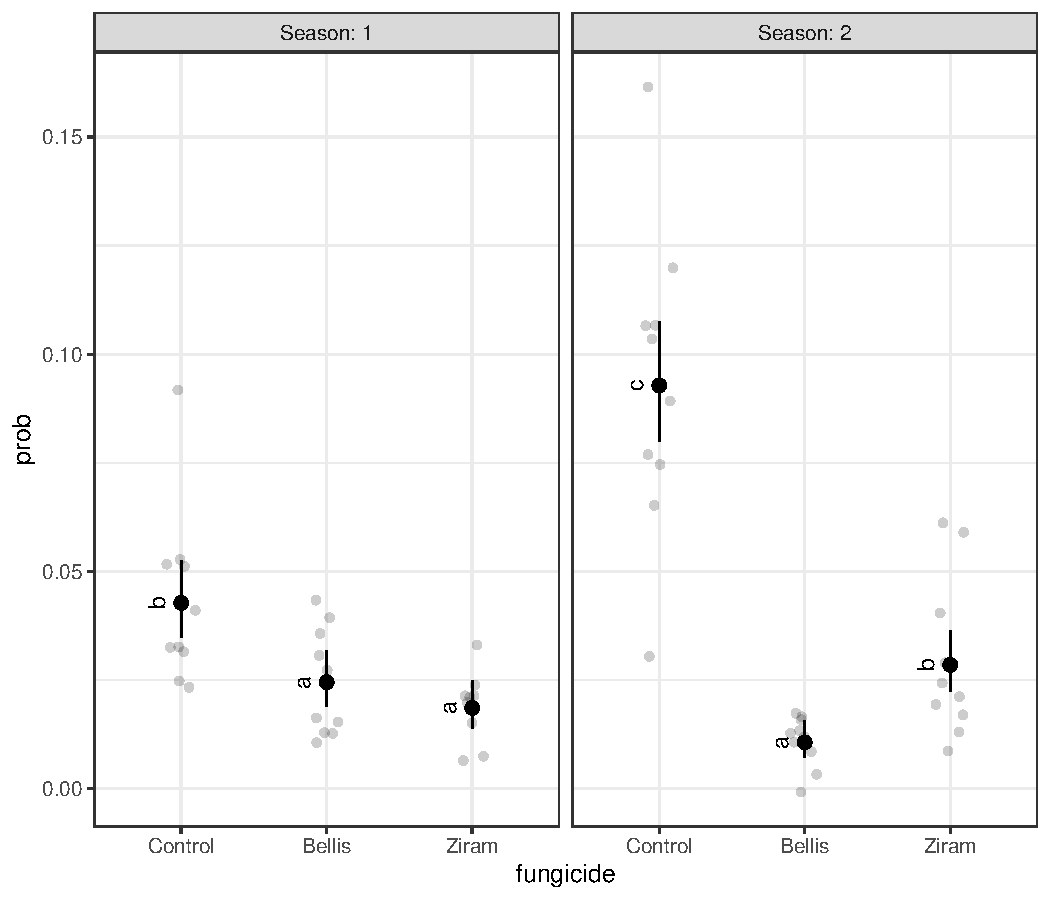
\includegraphics{in_field_files/figure-pdf/unnamed-chunk-8-1.pdf}

}

\end{figure}



\end{document}
